\documentclass{article}

\newif\ifanswers
\answerstrue % comment out to hide answers

\usepackage{fancyhdr} % Required for custom headers
\usepackage{lastpage} % Required to determine the last page for the footer
\usepackage{extramarks} % Required for headers and footers
\usepackage[usenames,dvipsnames]{color} % Required for custom colors
\usepackage{graphicx} % Required to insert images
\usepackage{listings} % Required for insertion of code
\usepackage{courier} % Required for the courier font
\usepackage{lipsum} % Used for inserting dummy 'Lorem ipsum' text into the template
\usepackage{enumerate}
\usepackage{booktabs}
\usepackage{amsmath, amsthm, amssymb}
\usepackage{caption}
\usepackage{subcaption}
\captionsetup[table]{skip=4pt}
\usepackage{framed}
\usepackage{bm}
\usepackage{float}
\usepackage[english]{babel}

\usepackage{style}
\usepackage{xcolor}
\graphicspath{{img/}} % set of paths to search for images
\usepackage{amsmath}
\usepackage{amsfonts}
\usepackage{amssymb}
\usepackage{hyperref}



\newenvironment{myitemize}
{ \begin{itemize}
		\setlength{\itemsep}{0pt}
		\setlength{\parskip}{0pt}
		\setlength{\parsep}{0pt}     }
	{ \end{itemize}                  } 


\usepackage[backend=bibtex]{biblatex}                                               
%\addbibresource{papers.bib}
\bibliography{papers.bib}

\usepackage{tikz}
\usetikzlibrary{positioning,patterns,fit}

\newcommand{\ifans}{\ifanswers \textbf{Solution: }}

% Margins
\topmargin=-0.45in
\evensidemargin=0in
\oddsidemargin=0in
\textwidth=6.5in
\textheight=9.0in
\headsep=0.25in

\linespread{1.1} % Line spacing

% Set up the header and footer
\pagestyle{fancy}
\rhead{\hmwkAuthorName} % Top left header
\lhead{\hmwkClass: \hmwkTitle} % Top center head
\lfoot{\lastxmark} % Bottom left footer
\cfoot{} % Bottom center footer
\rfoot{Page\ \thepage\ of\ \protect\pageref{LastPage}} % Bottom right footer
\renewcommand\headrulewidth{0.4pt} % Size of the header rule
\renewcommand\footrulewidth{0.4pt} % Size of the footer rule

\setlength\parindent{0pt} % Removes all indentation from paragraphs

%----------------------------------------------------------------------------------------
%	CODE INCLUSION CONFIGURATION
%----------------------------------------------------------------------------------------

\definecolor{MyDarkGreen}{rgb}{0.0,0.4,0.0} % This is the color used for comments
\lstloadlanguages{Python} % Load Perl syntax for listings, for a list of other languages supported see: ftp://ftp.tex.ac.uk/tex-archive/macros/latex/contrib/listings/listings.pdf
\lstset{language=Python, % Use Perl in this example
        frame=single, % Single frame around code
        basicstyle=\footnotesize\ttfamily, % Use small true type font
        keywordstyle=[1]\color{Blue}\bf, % Perl functions bold and blue
        keywordstyle=[2]\color{Purple}, % Perl function arguments purple
        keywordstyle=[3]\color{Blue}\underbar, % Custom functions underlined and blue
        identifierstyle=, % Nothing special about identifiers
        commentstyle=\usefont{T1}{pcr}{m}{sl}\color{MyDarkGreen}\small, % Comments small dark green courier font
        stringstyle=\color{Purple}, % Strings are purple
        showstringspaces=false, % Don't put marks in string spaces
        tabsize=5, % 5 spaces per tab
        %
        % Put standard Perl functions not included in the default language here
        morekeywords={rand},
        %
        % Put Perl function parameters here
        morekeywords=[2]{on, off, interp},
        %
        % Put user defined functions here
        morekeywords=[3]{test},
       	%
        morecomment=[l][\color{Blue}]{...}, % Line continuation (...) like blue comment
        numbers=left, % Line numbers on left
        firstnumber=1, % Line numbers start with line 1
        numberstyle=\tiny\color{Blue}, % Line numbers are blue and small
        stepnumber=5 % Line numbers go in steps of 5
}

% Creates a new command to include a perl script, the first parameter is the filename of the script (without .pl), the second parameter is the caption
\newcommand{\perlscript}[2]{
\begin{itemize}
\item[]\lstinputlisting[caption=#2,label=#1]{#1.pl}
\end{itemize}
}

%----------------------------------------------------------------------------------------
%	NAME AND CLASS SECTION
%----------------------------------------------------------------------------------------

\newcommand{\hmwkTitle}{Assignment \#2} % Assignment title
\newcommand{\hmwkClass}{CS\ 234 Winter 2019} % Course/class
\newcommand{\hmwkAuthorName}{} % Your name

%----------------------------------------------------------------------------------------
%	TITLE PAGE
%----------------------------------------------------------------------------------------

\title{
\vspace{-1in}
\textmd{\textbf{\hmwkClass:\ \hmwkTitle}}}
\author{}    
\date{} % Insert date here if you want it to appear below your name

\begin{document}

\maketitle
\vspace{-.5in}
\begin{framed}
{\bf Due date: 2/06 (Wed) 11:59 PM (23:59) PST}
\\[1em]
These questions require thought, but do not require long answers. Please be as concise as possible.
\\[1em]
We encourage students to discuss in groups for assignments. We ask
that you abide by the university Honor Code and that of the Computer Science department. If you have discussed the problems with others,
please include a statement saying who you discussed problems with. Failure to follow these instructions
will be reported to the Office of Community Standards. We reserve the right to run a fraud-detection software on your code. Please refer to \href{http://web.stanford.edu/class/cs234/index.html}{website}, Academic Collaboration and Misconduct section for details about collaboration policy.

\ \\[1em]
Please review any additional instructions posted on the assignment page. When you are ready to submit, please
follow the instructions on the course website. \textbf{Make sure you test your code using the
provided commands and do not edit outside of the marked areas.}
\\[1em]
You'll need to download the starter code and fill the appropriate functions following the instructions from the handout and the code's documentation. Training DeepMind's network on \texttt{Pong} takes roughly \textbf{12 hours on GPU}, so \textbf{please start early}! (Only a completed run will recieve full credit) We will give you access to an Azure GPU cluster. You'll find the setup instructions on the course assignment page.
\end{framed}
\section*{Introduction}

In this assignment we will implement deep Q learning, following DeepMind's paper (\cite{mnih2015human} and \cite{mnih-atari-2013}) that learns to play Atari from raw pixels. The purpose is to understand the effectiveness of deep neural network as well as some of the techniques used in practice to stabilize training and achieve better performance. You'll also have to get comfortable with Tensorflow. We will train our networks on the \texttt{Pong-v0} environment from OpenAI gym, but the code can easily be applied to any other environment. \\

In Pong, one player wins if the ball passes by the other player. Winning a game gives a reward of 1, while losing gives a negative reward of -1. An episode is over when one of the two players reaches 21  wins. Thus, the final score is between -21 (lost episode) or +21 (won episode). Our agent plays against a decent hard-coded AI player. Average human performance is $ -3 $ (reported in \cite{mnih-atari-2013}). If you go to the end of the homework successfully, you will train an AI agent with super-human performance, reaching at least +10 (hopefully more!).

\section{Test Environment (5 pts)}
Before running our code on Pong, it is crucial to test our code on a test environment. You should be able to run your models on CPU in no more than a few minutes on the following environment:

\begin{itemize}
\item $ 4 $ states: $ 0, 1, 2, 3 $
\item $ 5 $ actions: $ 0, 1, 2, 3, 4 $. Action $ 0 \leq i \leq 3 $ goes to state $ i $, while action $ 4 $ makes the agent stay in the same state.
\item Rewards: Going to state $ i $ from states 0, 1, and 3 gives a reward $R(i) $, where $R(0) = 0.1, R(1) = -0.2, R(2) = 0, R(3) = -0.1 $. If we start in state $ 2 $, then the rewards defind above are multiplied by $ - 10 $.  See Table~\ref{tab:TestEnv} for the full transition and reward structure. 
\item One episode lasts 5 time steps (for a total of 5 actions) and always starts in state $ 0 $ (no rewards at the initial state).        
\end{itemize}

\begin{center}
    \begin{tabular}{ | l | l | l | l |}  
    \hline
    State (s) & Action (a) & Next State (s') & Reward (R) \\ \hline
    0 & 0 & 0 & 0.1    \\ \hline
    0 & 1 & 1 & -0.2   \\ \hline
    0 & 2 & 2 & 0.0 \\ \hline
    0 & 3 & 3 & -0.1 \\ \hline
    0 & 4 & 0 & 0.1 \\ \hline
    1 & 0 & 0 & 0.1    \\ \hline
    1 & 1 & 1 & -0.2   \\ \hline
    1 & 2 & 2 & 0.0 \\ \hline
    1 & 3 & 3 & -0.1 \\ \hline
    1 & 4 & 1 & -0.2 \\ \hline
    2 & 0 & 0 & -1.0    \\ \hline
    2 & 1 & 1 & 2.0   \\ \hline
    2 & 2 & 2 & 0.0 \\ \hline
    2 & 3 & 3 & 1.0 \\ \hline
    2 & 4 & 2 & 0.0 \\ \hline
    3 & 0 & 0 & 0.1    \\ \hline
    3 & 1 & 1 & -0.2   \\ \hline
    3 & 2 & 2 & 0.0 \\ \hline
    3 & 3 & 3 & -0.1 \\ \hline
    3 & 4 & 3 & -0.1 \\ \hline    
    \end{tabular}
\captionof{table}{Transition table for the Test Environment} \label{tab:TestEnv} 
\end{center}

An example of a path (or an episode) in the test environment is shown in Figure \ref{fig:test_env}, and the trajectory can be represented in terms of $s_t, a_t, R_t$ as: 
$s_0 = 0, a_0=1, R_0 = -0.2, s_1=1, a_1=2, R_1 = 0, s_2=2, a_2=4, R_2 = 0, s_3=2, a_3=3, R_3 = (-0.1)*(-10) = 1, s_4=3, a_4=0, R_4 = 0.1, s_5=0 $.

\begin{figure}[H]
  \centering
  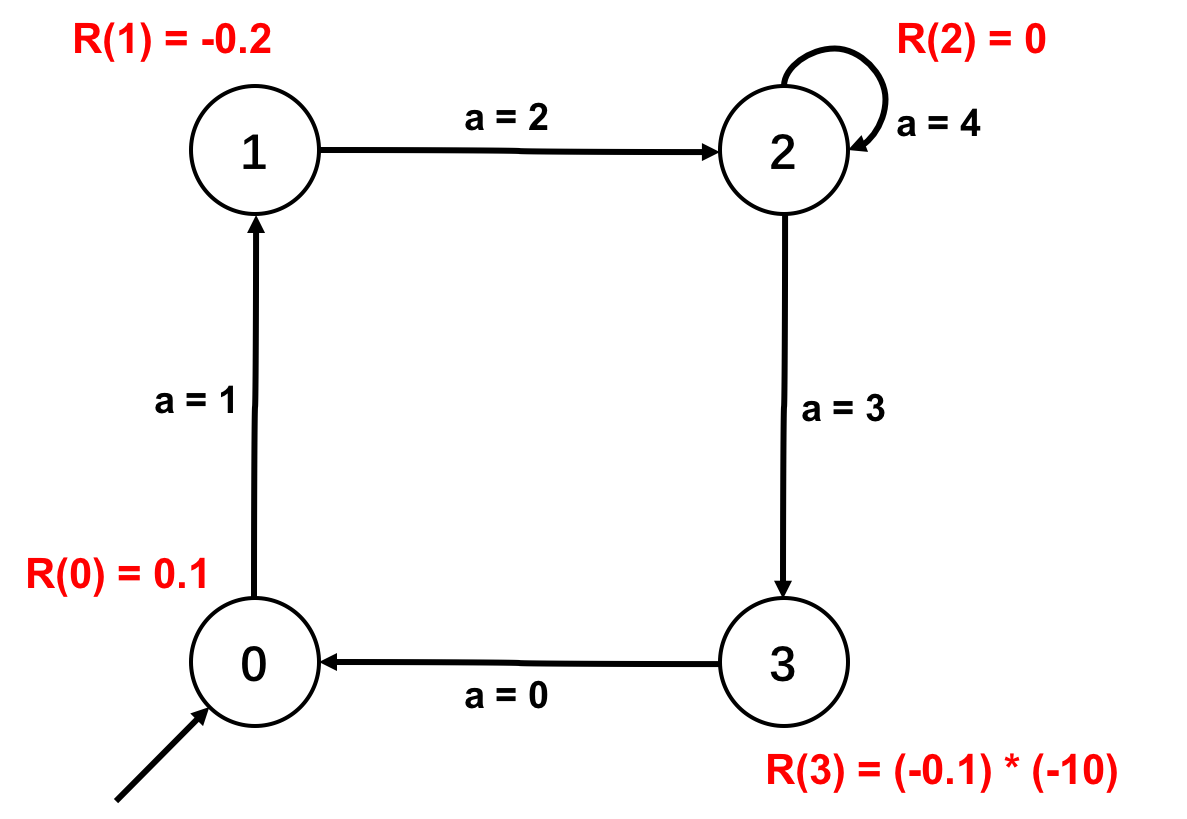
\includegraphics[width=.45\linewidth]{test_env}
  \caption{Example of a path in the Test Environment}
  \label{fig:test_env}
\end{figure}

\begin{enumerate}
\item (\textbf{written} 5pts) What is the maximum sum of rewards that can be achieved in a single episode in the test environment, assuming $\gamma = 1$?
\end{enumerate}


\section{Q-learning (12 pts)}\label{q-learn}

\paragraph{Tabular setting}
In the \emph{tabular setting}, we maintain a table $ Q(s, a) $ for each tuple state-action. Given an experience sample $ (s, a, r, s') $, our update rule is
\begin{equation}
\label{eq1}
\begin{split}
Q(s,a) &= Q(s,a) + \alpha\left(r+\gamma \max_{a' \in A}Q\left(s',a' \right) - Q\left(s, a\right)\right),
\end{split}
\end{equation}
where $\alpha \in \mathbb{R}$ is the learning rate, $ \gamma $ the discount factor. 

\paragraph{Approximation setting} 
Due to the scale of Atari environments, we cannot reasonably learn and store a Q value for each state-action tuple. We will instead represent our Q values as a function $ \hat{q}(s, a, \textbf{w}) $ where $ \textbf{w} $ are parameters of the function (typically a neural network's weights and bias parameters). In this \emph{approximation setting}, our update rule becomes
\begin{equation}
\label{eq2}
\textbf{w} = \textbf{w} + \alpha\left(r+\gamma \max_{a' \in A} \hat{q}\left(s',a', \textbf{w} \right) - \hat{q}\left(s, a, \textbf{w} \right)\right) \nabla_{\textbf{w}}\hat{q}(s,a, \textbf{w}).
\end{equation}
In other words, we are try to minimize
\begin{equation}
L(\textbf{w}) = \mathbf{E}_{s,a,r,s'}{\left[r+\gamma \max_{a' \in A}\hat{q}\left(s',a', \textbf{w} \right) - \hat{q}(s,a, \textbf{w})\right]}^2
\end{equation}

\paragraph{Target Network}
DeepMind's paper \cite{mnih2015human} \cite{mnih-atari-2013} maintains two sets of parameters, $\textbf{w}$ (to compute $ \hat{q}(s, a)$) and $\textbf{w}^-$ (target network, to compute $ \hat{q}(s', a') $) such that our update rule becomes
\begin{equation}
\textbf{w} = \textbf{w} + \alpha\left(r+\gamma \max_{a' \in A}\hat{q}\left(s',a', \textbf{w}^- \right) - \hat{q}\left(s, a, \textbf{w} \right)\right) \nabla_{\textbf{w}} \hat{q}(s,a, \textbf{w}).
\end{equation}
The target network's parameters are updated with the Q-network's parameters occasionally and are kept fixed between individual updates. Note that when computing the update, we don't compute gradients with respect to $ \textbf{w}^- $ (these are considered fixed weights).

\paragraph{Replay Memory}
As we play, we store our transitions $ (s, a, r, s') $ in a buffer. Old examples are deleted as we store new transitions. To update our parameters, we \emph{sample} a minibatch from the buffer and perform a stochastic gradient descent update.

\paragraph{$\epsilon$-Greedy Exploration Strategy}
During training, we use an $ \epsilon $-greedy strategy. DeepMind's paper \cite{mnih2015human} \cite{mnih-atari-2013} decreases $ \epsilon $ from $ 1 $ to $ 0.1 $ during the first million steps. At test time, the agent choses a random action with probability $ \epsilon_{soft} = 0.05 $.\\

There are several things to be noted:
\begin{itemize}
\item In this assignment, we will update $ \textbf{w} $ every \texttt{learning\_freq} steps by using a \texttt{minibatch} of experiences sampled from the replay buffer.

\item DeepMind's deep Q network takes as input the state $ s $ and outputs a vector of size = number of actions. In the \texttt{Pong} environment, we have $ 6 $ actions, thus
$ \hat{q}(s, \textbf{w}) \in \mathbb{R}^{6} $.    
\item The input of the deep Q network is the concatenation $ 4 $ consecutive steps, which results in an input after preprocessing of shape $ (80 \times 80 \times 4) $.
\end{itemize}

We will now examine these assumptions and implement the epsilon-greedy strategy.

\begin{enumerate}
\item (\textbf{written} 3pts) What is one benefit of using experience replay?

\item (\textbf{written} 3pts) What is one benefit of the target network?

\item (\textbf{written} 3pts) What is one benefit of representing the $Q$ function as $ \hat{q}(s, \textbf{w}) \in \mathbb{R}^{K} $

\item (\textbf{coding} 3pts) Implement the \texttt{get\_action} and \texttt{update} functions in \texttt{q1\_schedule.py}. Test your implementation by running \texttt{python q1\_schedule.py}.
\end{enumerate}

\section{Linear Approximation (26 pts)}
\begin{enumerate}
\item (\textbf{written} 3pts) Show that Equations (\ref{eq1}) and (\ref{eq2}) from section \ref{q-learn} above are exactly the same when $\hat{q}(s,a, \textbf{w}) = \textbf{w}^Tx(s,a)$, where $\textbf{w} \in \mathbb{R}^{\vert S\vert \vert A\vert }$ and $x: S \times A \rightarrow \mathbb{R}^{\vert S\vert \vert A\vert }$ such that
\[
    x(s,a)_{s',a'}=\left\{
                \begin{array}{ll}
                  1 & \text{ if } s'=s, a'=a\\
                  0 & \text{otherwise}\\
                \end{array}
              \right.
  \]


 for all $(s, a) \in S \times A$, $x(s,a)$ is a vector of length $|S||A|$ where the element corresponding to $s^\prime \in S, a^\prime \in A$ is 1 when $s^\prime = s, a^\prime = a$ and is 0 otherwise.

 \item (\textbf{written} 3pts) Derive the gradient with regard to the value function parameter $\textbf{w} \in \mathbb{R}^n$ given $\hat{q}(s,a, \textbf{w}) = \textbf{w}^Tx(s,a)$ for any function $ x (s, a) \mapsto x \in \mathbb{R}^n $ and write the update rule for $ \textbf{w} $.
 
 \item (\textbf{coding} 15pts) We will now implement linear approximation in Tensorflow. This question will setup the whole pipeline for the remiander of the assignment. You'll need to implement the following functions in \texttt{q2\_linear.py} (pleasd read through\texttt{q2\_linear.py}) :
\begin{itemize}
	\item \texttt{add\_placeholders\_op}
	\item \texttt{get\_q\_values\_op}
	\item \texttt{add\_update\_target\_op}
	\item \texttt{add\_loss\_op}
	\item \texttt{add\_optimizer\_op}
\end{itemize}
Test your code by running \texttt{python q2\_linear.py} \textbf{locally on CPU}.  This will run linear approximation with Tensorflow on the test environment.  Running this implementation should only take a minute or two.
 
 \item (\textbf{written} 5pts) Do you reach the optimal achievable reward on the test environment? Attach the plot \texttt{scores.png} from the directory \texttt{results/q2\_linear} to your writeup.
\end{enumerate}

\section{Implementing DeepMind's DQN (15 pts)}

\begin{enumerate}

\item (\textbf{coding} 10pts) Implement the deep Q-network as described in \cite{mnih2015human} by implementing \texttt{get\_q\_} \texttt{values\_op} in \texttt{q3\_nature.py}. The rest of the code inherits from what you wrote for linear approximation. Test your implementation \textbf{locally on CPU} on the test environment by running \texttt{python q3\_nature.py}.  Running this implementation should only take a minute or two.

\item (\textbf{written} 5pts) Attach the plot of scores, \texttt{scores.png}, from the directory \texttt{results/q3\_nature} to your writeup. Compare this model with linear approximation. How do the final performances compare? How about the training time? 

\end{enumerate}

\section{DQN on Atari (27 pts)}

The Atari environment from OpenAI gym returns observations (or original frames) of size $ (210 \times 160 \times 3) $, the last dimension corresponds to the RGB channels filled with values between $ 0 $ and $ 255 $ (\texttt{uint8}). Following DeepMind's paper \cite{mnih2015human}, we will apply some preprocessing to the observations:   
\begin{myitemize}
\item Single frame encoding: To encode a single frame, we take the maximum value for each pixel color value over the frame being encoded and the previous frame. In other words, we return a pixel-wise max-pooling of the last 2 observations.     
\item Dimensionality reduction: Convert the encoded frame to grey scale, and rescale it to $(80 \times 80 \times 1)$. (See Figure \ref{fig:pong_env})     
\end{myitemize}

The above preprocessing is applied to the 4 most recent observations and these encoded frames are stacked together to produce the input (of shape $(80 \times 80 \times 4)$) to the Q-function. Also, for each time we decide on an action, we perform that action for 4 time steps. This reduces the frequency of decisions without impacting the performance too much and enables us to play 4 times as many games while training. You can refer to the \textit{Methods Section} of \cite{mnih2015human} for more details.       \\  

\begin{figure}[H]
\centering
\begin{subfigure}[b]{.5\textwidth}
  \centering
  
\includegraphics[width=.25\linewidth]{pong}
  \caption{Original input $ (210 \times 160 \times 3) $ with RGB colors}
  \label{fig:pong}
\end{subfigure}%
\begin{subfigure}[b]{.5\textwidth}
  \centering
  
\includegraphics[width=.15\linewidth]{pong_grey}
  \caption{After preprocessing in grey scale of shape $ (80 \times 80 \times 1 ) $}
  \label{fig:pong_grey}
\end{subfigure}
\caption{\texttt{Pong-v0} environment}
\label{fig:pong_env}
\end{figure}

\begin{enumerate}
\item (\textbf{written} 2pts) Why do we use the last $ 4 $ time steps as input to the network for playing Atari games?   

\item (\textbf{written} 5pts) What's the number of parameters of the DQN model (for \texttt{Pong}) if the input to the Q-network is a tensor of shape $ (80, 80, 4) $ and we use "SAME" padding? How many parameters are required for the linear Q-network, assuming the input is still of shape $(80, 80, 4)$?  How do the number of parameters compare between the two models?

\item (\textbf{coding and written} 5pts). Now, we're ready to train on the Atari \texttt{Pong-v0} environment. First, launch linear approximation on pong with \texttt{python q4\_train\_atari\_linear.py} \textbf{on Azure's GPU}. This will train the model for 500,000 steps and should take approximately an hour.  What do you notice about the performance?

\item (\textbf{coding and written} 10 pts). In this question, we'll train the agent with DeepMind's architecture on the Atari \texttt{Pong-v0} environment. Run \texttt{python q5\_train\_atari\_nature.py} \textbf{on Azure's GPU}.  This will train the model for 5 million steps and should take around \textbf{12 hours}.  Attach the plot \texttt{scores.png} from the directory \texttt{results/q5\_train\_atari\_nature} to your writeup. 
You should get a score of around 13-15 after 5 million time steps.  As stated previously, the Deepmind paper claims average human performance is $ -3 $.


As the training time is roughly 12 hours, you may want to check after a few epochs that your network is making progress.  The following are some training tips:

\begin{myitemize}
\item If you terminate your terminal session, the training will stop.  In order to avoid this, you should use \texttt{screen} to run your training in the background.
\item The evaluation score printed on terminal should start at -21 and increase.
\item The max of the q values should also be increasing
\item The standard deviation of q shouldn't be too small. Otherwise it means that all states have similar q values
\item You may want to use Tensorboard to track the history of the printed metrics. You can monitor your training with Tensorboard by typing the command \texttt{tensorboard --logdir=results} and then connecting to \texttt{ip-of-you-machine:6006}.  Below are our Tensorboard graphs from one training session:
\end{myitemize}

\begin{figure}[H]
\centering
	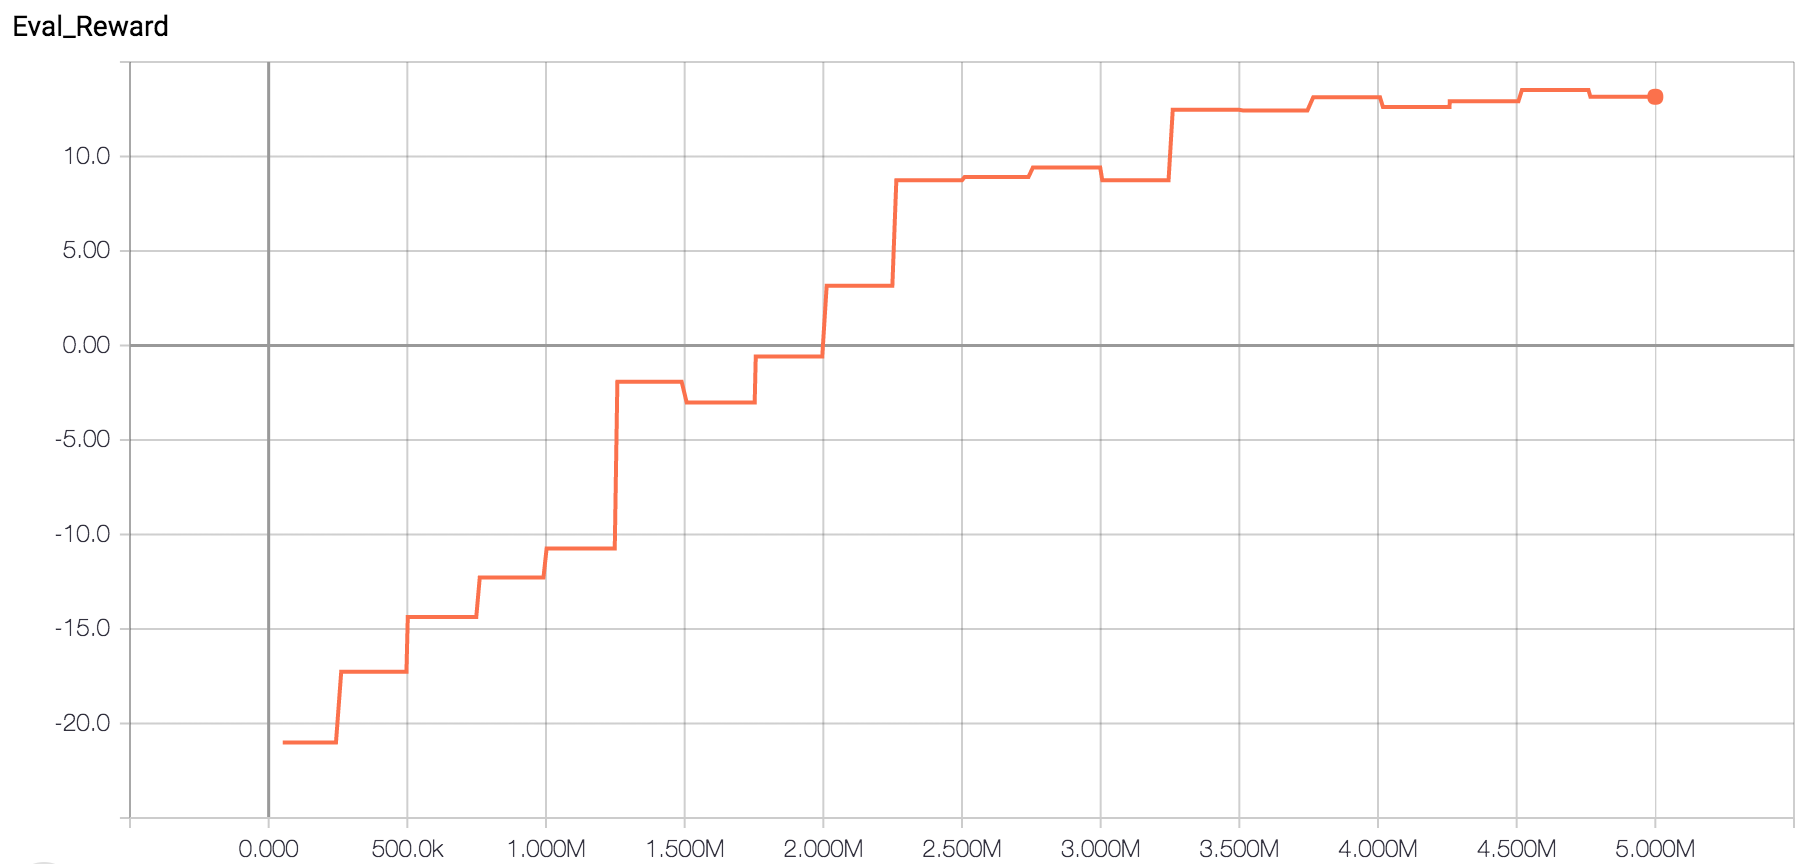
\includegraphics[width=.4\linewidth]{Eval_R.png}
	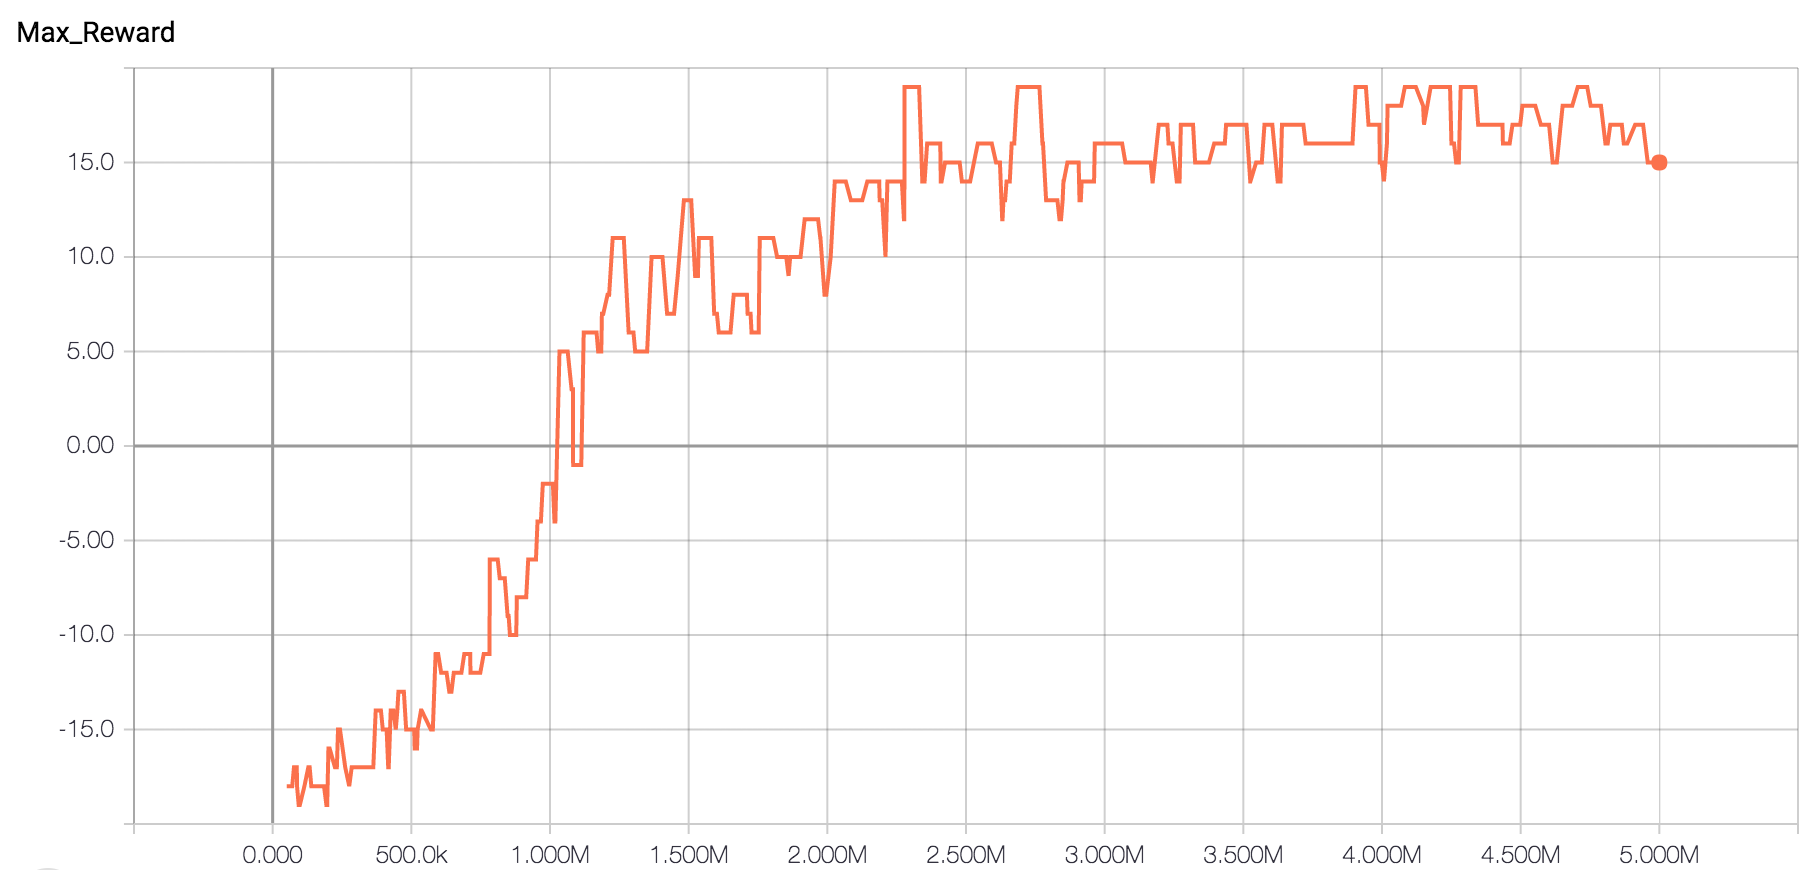
\includegraphics[width=.4\linewidth]{Max_R.png}
	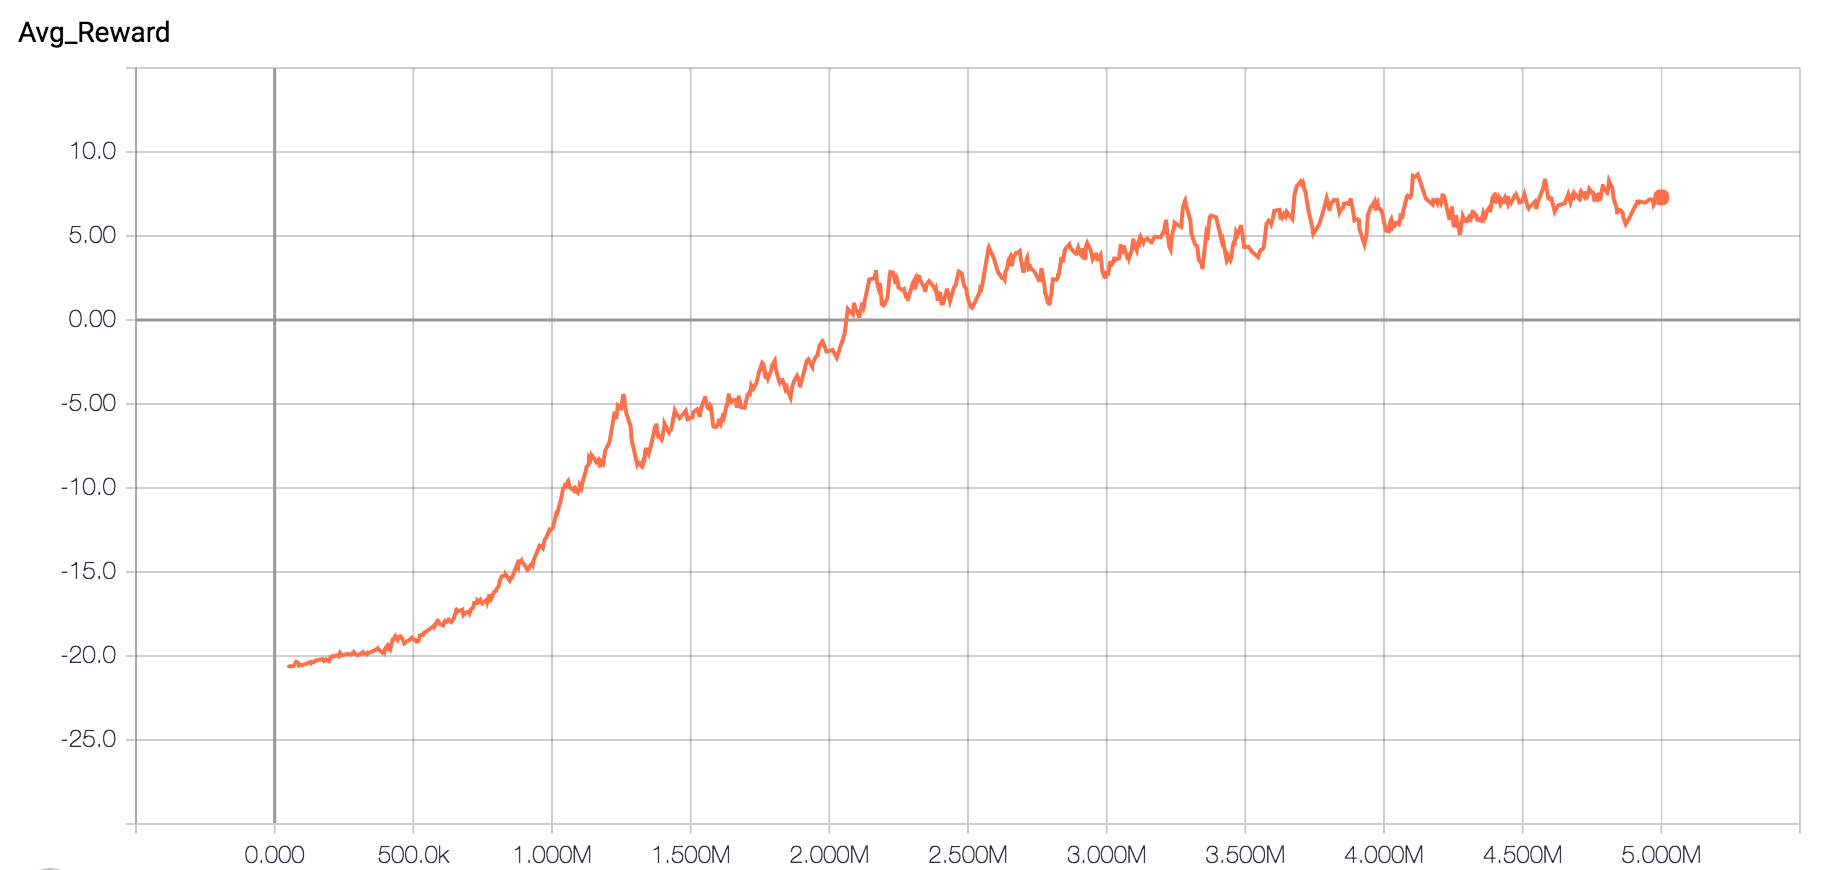
\includegraphics[width=.4\linewidth]{Avg_R.png}
	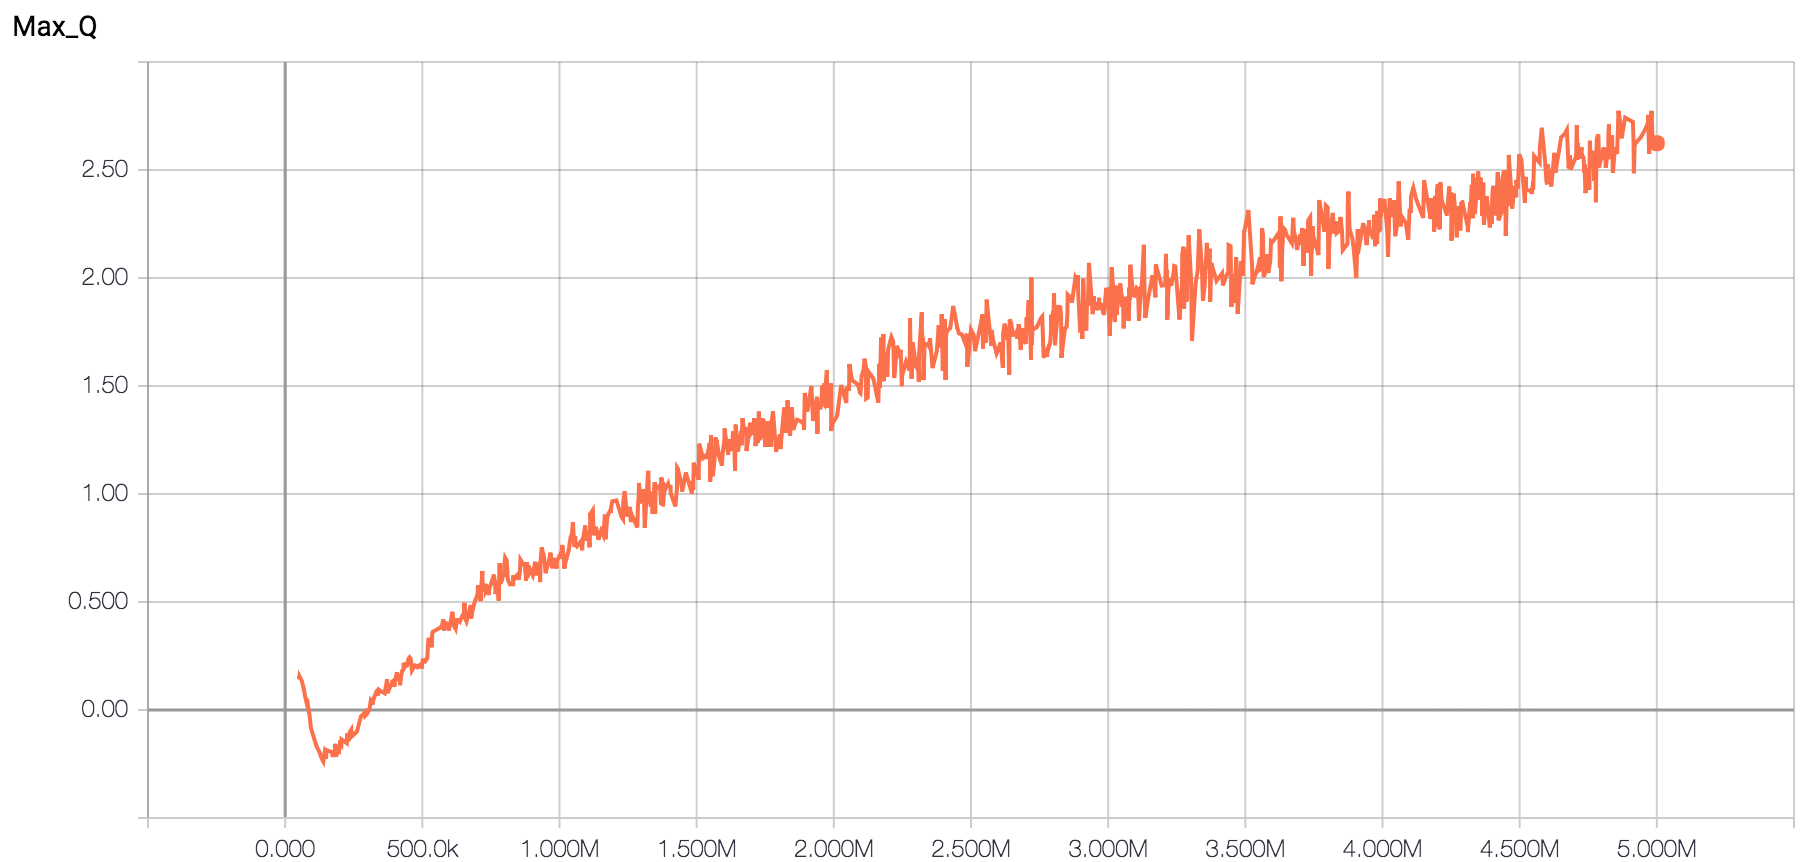
\includegraphics[width=.4\linewidth]{Max_Q.png}
\end{figure}

\item (\textbf{written} 5pts) Compare the performance of the DeepMind architecure with the linear Q-network approximation. How can you explain the gap in performance?
\end{enumerate}

\section{Real world RL with neural networks (10 pts)}
Given a stream of batches of $n$ environment interactions $(s_i,a_i,r_i,s'_i)$ we want to learn the optimal value function using a neural network. The underlying MDP has a finite sized action space.
\begin{enumerate}
\item[1.] (\textbf{written} 4pts) Your friend first suggests the following approach
\begin{enumerate}
    \item Initialize parameters \(\phi\) of neural network \(V_\phi\)
    \item For each batch of $k$ tuples $(s_i,a_i,r_i,s'_i)$ do Stochastic Gradient Descent with loss function \(\sum_{i=0}^k|y_i-V_\phi(s_i)|^2\) where \(y_i = \max_{a_i} [r_i+\gamma V_\phi(s'_i)]\)
\end{enumerate}
What is the problem with this approach? (Hint: Think about the type of data we have)
\item[2.] (\textbf{written} 3pts) Your friend now suggests the following
\begin{enumerate}
    \item Initialize parameters \(\phi\) of neural network for state-action value function \(Q_\phi(s,a)\)
    \item For each batch of $k$ tuples $(s_i,a_i,r_i,s'_i)$ do Stochastic Gradient Descent with loss function \(\sum_{i=0}
    ^k|y_i-Q_\phi(s_i,a_i)|^2\) where \(y_i = r_i+\gamma V(s'_i)\)
\end{enumerate}
Now as we just have the network $Q_\phi(s,a)$ how would you determine $V(s)$ needed for the above training procedure?
\item[3.] (\textbf{written} 3pts) Is the above method of learning the $Q$ network guaranteed to give us an approximation of the optimal state action value function?
\end{enumerate}

\end{document}
